\documentclass[10pt,a4paper]{amsart}

\usepackage[]{graphicx}
\usepackage[]{hyperref}
\usepackage[]{physics}
\usepackage[]{listings}
\usepackage[utf8]{inputenc}
\usepackage[toc,page]{appendix}
\usepackage[dvipsnames]{xcolor}
\usepackage{tikz}


\definecolor{mygray}{gray}{0.9}

\lstset{
	frame = single,
	language = C++,
	showstringspaces = false,
	tabsize = 2,
	otherkeywords = {self},
	keywordstyle = \color{Maroon},
	identifierstyle=\color{olive},
 	stringstyle=\color{orange},
 	backgroundcolor=\color{mygray},
 	breaklines = true
}

\title[Ising model in 2d]{The Ising model in two dimensions \\ 
	\hrulefill\small{ FYS3150: Computational Physics }\hrulefill}
	
\author[Winther-Larsen]{Sebastian G. Winther-Larsen \\
\href{https://github.com/gregwinther/FYS3150/}{\texttt{github.com/gregwinther}}}
	
\date{\today}

\begin{document}

\begin{titlepage}
\begin{abstract}
Ising model in 2D. Metropolis algorithm etc. Shit goes down.
\end{abstract}
\maketitle
\tableofcontents
\end{titlepage}

\section{Introduction}

\section{Theory}
The model we will employ in this study of phase transitions at finite temperature for magnetic systems is the Ising model, named after Ernst Ising who solved a one-dimensional variant of the model\cite{Ising}. The two-dimensional square lattice model, employed herein, was given an analytic description much later by Lars Onsager\cite{Onsager}.

\subsection{The general Ising model}
Let $\Lambda$ be a set of lattice positions, each with adjacent positions, forming a $d$-dimensional lattice. For each lattice site, $k \in \Lambda$, there is a discrete variable $\sigma_k \in \{+1,-1\}$, representing the spin of the site, $\uparrow$ and $\downarrow$, respectively. A spin configuration $\sigma$ is a specific spin configuration of the lattice.

For two adjacent sites, $i,j \in \Lambda$, one has an interaction $J_{ij}$. A site $j \in \Lambda$ will also have an external magnetic field $h_j$ interacting with it. The energy of a specific system is given by the following Hamiltonian
\begin{equation}
\label{eq:IsingHamilton}
E = H(\sigma)= -\sum_{\ev{ik}}J_{ij}\sigma_i \sigma_j - \mu \sum_j h_j \sigma_j,
\end{equation}
where the first sum is over pairs of adjacent spins. The notation $\ev{ij}$ indicates that sites $i$ and $j$ are nearest neighbours. In the second sum, $\mu$ is the magnetic moment.

The probability of a certain configurations is given by the Boltzmann distribution
\begin{equation}
\label{eq:Boltzmann}
P_\beta(\sigma) = \frac{e^{-\beta H(\sigma)}}{Z_\beta}
\end{equation}
where $Z_\beta$ is the partition function acting as a normalisation constant, and $\beta=(k_BT)^{-1}$. This would mean that by increasing the temperature $T$, finding the system in one particular configuration decreases. It must be so, because with a relatively higher temperature, one would expect previously unfavourable configuration to become more feasible.

There are two important expected values that are important in order to characterise a magnetic system. The \emph{mean energy} of the system is
\begin{equation}
\label{eq:meanenergy}
\ev{E} = \sum_{i=1}^ME_iP_\beta(\sigma) = \frac{1}{Z}\sum_{i=1}^ME_ie^{-\beta E_i},
\end{equation}
and the \emph{mean magnetisation} is
\begin{equation}
\label{eq:meanmagnet}
\ev{\mathcal{M}} = \sum_{i=1}^M\mathcal{M}_iP_\beta(\sigma) = \frac{1}{Z}\sum_{i=1}^M\mathcal{M}_ie^{\beta E_i},
\end{equation}
where $\mathcal{M}_i = \sum_{j \in \Lambda}\sigma_j$ for all configurations $\sigma$, and $M$ denotes the number of possible configurations. Another quantity of interest is \emph{magnetic susceptibility} $\chi$ which tells us how much an extensive parameter changes when an intensive parameter increases. It is given by
\begin{equation}
\label{eq:susceptibility}
\chi = \frac{1}{k_BT}(\ev{\mathcal{M}^2} - \ev{\mathcal{M}}^2).
\end{equation}
The \emph{heat capacity}, at constant volume, is given by
\begin{equation}
\label{eq:heatcap}
C_V = \frac{1}{k_BT^2}(\ev{E^2}-\ev{E}^2)
\end{equation}

The minus sign on each term of the Hamiltonian $H(\sigma)$ in equation \ref{eq:IsingHamilton} is conventional. By this sign convention, the Ising model can be classified according to the sign of the interaction. If, for all pairs $i,j$:
\begin{itemize}
\item $J_{ij} > 0$, the interaction is ferromagnetic,
\item $J_{ij} < 0$, the interaction is anti-ferromagnetic,
\item $J_{ij} = 0$, the spins are non-interacting.
\end{itemize}
In a ferromagnetic Ising model, spins desire to be aligned: the configurations in which adjacent spins are of the same sign have higher probability. In an anti-ferromagnetic model, adjacent spins tend to have opposite signs.

\subsection{Simplified ferromagnetic Ising model}
The general Ising model, as described above, will not be used in this study, but a much simpler version of it. Firstly, we will examine a system with no external magnetic field, as was originally solved analytically by Onsager\cite{Onsager}. Because the second sum in the Hamiltonian in equation \ref{eq:IsingHamilton} is zero, and we are left with
\begin{equation}
\label{eq:IsingHamSimple1}
E = H(\sigma) = -\sum_{\ev{ik}}J_{ij}\sigma_i\sigma_j.
\end{equation} 
Secondly, we assume that the coupling constant $J_{ij}$, that describe the interaction of a spin with its neighbour, to be constant. That is $J_{ij} = J \forall i,j \in \Lambda$ and equation \ref{eq:IsingHamSimple1} is simplified further to
\begin{equation}
\label{eq:IsingHamSimple2}
E = H(\sigma) = -J \sum_{\ev{ik}}\sigma_i\sigma_j
\end{equation}

In this study, we will assume that we have a ferromagnetic ordering, id est  $J>0$. This means that neighbouring spins are aligned, because it would lead to lower energy. It is easy to see why it must be so, as $\sigma_i\sigma_j=1$ whenever spin $i$ and $j$ have the same sign.

\subsection{Example: $2\times2$ Ising model}
It would be beneficial to test the waters of the ocean of the vast ocean that is the Ising model, by a two-dimensional model with lattice dimension $L=2$ and periodic boundary conditions. This model has $s=2^4=16.$ different configurations $\sigma$. The energy of a given configuration would be
\begin{equation*}
E_i = -J \sum_{\ev{kl}}^4 \sigma_k \sigma_l.
\end{equation*}

Figure \ref{fig:2by2lattice} shows an arbitrary configuration of a $2\times2$ spin lattice. The energy for this configuration is
\begin{equation*}
E_i = -J((+1)(-1)+(+1)(-1)+(+1)(-1)+(+1)(-1)) = 8J
\end{equation*}
which happens to be the highest energy possible for the system. When all spins are parallel we see that $E_i=-8J$ which is the lowest energy possible. If only one spin would differ from the others, the energy would be $E_i = 0$ and so on. Of the $16$ possible configurations, several will have degeneracies ($\Omega(E_i)$), which corresponds to the number of configurations with the same energy. Moreover, the magnetisation of a particular configuration is simply the sum of the spins and is easy to calculate. All the possible configurations of this system can be found in table \ref{tab:2by2lattice}.

\begin{figure}[h]
	\centering
	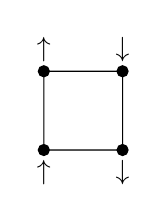
\begin{tikzpicture}
	\filldraw 	(0,0) circle(2pt) node[align=left, below]{$\uparrow$}-- 
				(0,1) circle(2pt) node[align=left, above]{$\uparrow$}-- 
				(1,1) circle(2pt) node[align=right, above]{$\downarrow$}-- 
				(1,0) circle(2pt) node[align=right, below]{$\downarrow$}-- (0,0);
	\end{tikzpicture}
	\caption{Sample $2\times2$ spin lattice.}
	\label{fig:2by2lattice}
\end{figure}

\begin{table}
	\centering
	\caption{All possible configurations of a $2\times2$ Ising model}
	\begin{tabular}{cccc} \hline
	No of $\uparrow$ & $\Omega(E_i)$ & $E_i$ & $\mathcal{M}_i$ \\ \hline
	$4$ & $1$ & $-8J$ & $4$  \\
	$3$ & $4$ & $0$   & $2$ \\
	$2$ & $4$ & $0$   & $0$  \\
	$2$ & $2$ & $8J$  & $0$  \\
	$1$ & $4$ & $0$   & $-2$ \\
	$0$ & $1$ & $-8J$ & $-4$ \\ \hline
	\end{tabular}
	\label{tab:2by2lattice}
\end{table}

Now to compute the physical quantities as discussed above, expected value for energy $\ev{E}$, expected value for magnetisation $\ev{\mathcal{M}}$, expected value for specific heat $\ev{C_V}$, and susceptibility $\chi$. For the $2\times2$ Ising model these quantities have closed form expressions. The partition function for the system is given by
\begin{equation}
\label{2by2partition}
Z = \sum_{i=1}^16 e^{-\beta E_i} = e^{\beta8J} + 12 + 2e^{-\beta8J} + e^{\beta8J} = 4\cosh(\beta8J) + 12
\end{equation}
The expected energy is
\begin{equation}
\label{2by2expectedE}
\ev{E} = -\frac{\partial}{\partial\beta} \ln Z = -\frac{\partial}{\partial \beta}\ln(4\cosh(\beta J) + 12)
 = -8J \frac{\sinh(8\beta J)}{\cosh(8\beta J) + 3}.
\end{equation}
The mean magnetisation for this system is easiest to compute with equation \ref{eq:meanmagnet}, merely adding all possible states and dividing by the partition function.
\begin{equation}
\label{eq:2by2meanmagnet}
\ev{\mathcal{M}}= \frac{1}{Z}(-4e^{8\beta J} - 8e^0 + 8e^0 +8e^{8\beta J}) = 0
\end{equation}
the expected absolute magnetisation, on the other hand, becomes
\begin{equation}
\label{eq:2by2absmeanmagnet}
\ev{\abs{\mathcal{M}}} = \frac{1}{Z}(4e^{8\beta J} + 8e^0 + 8e^0 + 4e^{8\beta J}) = \frac{4 +2 e^{8\beta J}}{\cosh(8\beta J) +3}.
\end{equation}
The expected value for specific heat is
\begin{equation}
\label{eq:2by2specificheat}
\ev{C_V} = \frac{1}{k_bT^2}\frac{\partial^2}{\partial\beta^2}
\end{equation}
inserting equation \ref{2by2expectedE} gives
\begin{align*}
\ev{C_V} 	&= -\frac{1}{k_BT^2}\frac{\partial}{\partial\beta}\left(-8J\frac{\sinh(8\beta J)}{\cosh(8\beta J)+3} \right) \\
			&= \frac{1}{k_BT^2}\left(\frac{64J^2\cosh(8\beta J)}{\cosh(8\beta J)+3}-\frac{64J^2\sinh^2(8\beta J)}{(\cosh(8\beta J)+3)^2}\right) \\
			&= \frac{1}{k_BT^2}\frac{64J^2}{\cosh(8\beta J) + 3}\left(\cosh(8\beta J) - \frac{\sinh^2(8\beta J)}{\cosh(8\beta J) +3} \right)
\end{align*}

The susceptibility $\chi$ of a thermodynamic system is easy to compute if one knows what the variance of magnetisation, $\sigma_{\mathcal{M}}^2)$, is. Rewriting equation \ref{eq:susceptibility} gives
\begin{equation}
\label{eq:susceptibility2}
\chi = \frac{1}{k_BT}\sigma_{\mathcal{M}}^2.
\end{equation}
Using equations \ref{eq:2by2meanmagnet} and \ref{eq:2by2absmeanmagnet} one can deduce that the variance of the magnetisation must be
\begin{equation}
\label{eq:2by2magnetvar}
\sigma_{\mathcal{M}}^2 = \ev{\mathcal{M}^2} - \ev{\mathcal{M}}^2 = \frac{32}{Z}(e^{8\beta J} +1) - 0 = \frac{8(e^{8\beta J} + 1)}{\cosh(8\beta J) + 3}.
\end{equation}
Inserting \ref{eq:2by2magnetvar} into \ref{eq:susceptibility2} yields the susceptibility for the system
\begin{equation}
\label{eq:2by2susceptibility}
\chi = \frac{8(e^{8\beta J}+1)}{k_BT(\cosh(8\beta T) + 3)}
\end{equation}

Bear in mind that $\beta = \frac{1}{k_BT}$, and that all the quantities computed are functions of $T$. The results computed here can be used as comparison for numerical computations.

\section{Algorithm}

\section{Results}

\section{Discussion}

\section{Conclusion}

\begin{thebibliography}{9}

\bibitem{Ising} Ising, E., Beitrag zur Theorie des Ferromagnetismus,
	\emph{Z. Phys.,} 31, pp. 253-258 (1925).

\bibitem{Onsager} Onsager, L., Crystal statistics. I. A two-dimensional model with an order-disorder transition,
	\emph{Physical Review,} Series II, 65 (3-4), pp. 117-149 (1944).

\end{thebibliography}

\end{document}